\documentclass[11pt,a4paper]{article}

\usepackage{amsmath,amssymb,mathtools}
\usepackage{amsthm}
\usepackage{centernot}
\usepackage{enumitem}
\usepackage{booktabs}
\usepackage{graphicx}
\usepackage{float}
\usepackage{algorithm}
\usepackage{algpseudocode}
\usepackage[colorlinks=true,citecolor=blue,linkcolor=blue,urlcolor=blue]{hyperref}
\usepackage[margin=2.5cm]{geometry}

% Theorem environments
\newtheorem{theorem}{Theorem}[section]
\newtheorem{lemma}[theorem]{Lemma}
\newtheorem{proposition}[theorem]{Proposition}
\newtheorem{corollary}[theorem]{Corollary}
\newtheorem{hypothesis}[theorem]{Hypothesis}
\newtheorem{algorithm2}[theorem]{Algorithm}
\theoremstyle{definition}
\newtheorem{definition}[theorem]{Definition}
\newtheorem{example}[theorem]{Example}
\theoremstyle{remark}
\newtheorem{remark}[theorem]{Remark}



\DeclareMathOperator{\Tr}{Tr}
\DeclareMathOperator{\Dom}{Dom}
\DeclareMathOperator{\ad}{ad}
\DeclareMathOperator{\id}{id}
\DeclareMathOperator{\diag}{diag}
\DeclareMathOperator{\supp}{supp}
\DeclareMathOperator{\EP}{EP}
\newcommand{\inner}[2]{\langle #1, #2 \rangle}
\newcommand{\R}{\mathbb{R}}
\newcommand{\C}{\mathbb{C}}
\newcommand{\N}{\mathbb{N}}
\newcommand{\Z}{\mathbb{Z}}
\newcommand{\HH}{\mathcal{H}}
\newcommand{\FF}{\mathcal{F}}
\newcommand{\BB}{\mathcal{B}}
\newcommand{\DD}{\mathcal{D}}
\newcommand{\TT}{\mathcal{T}}
\newcommand{\LL}{\mathcal{L}}
\newcommand{\abs}[1]{\lvert #1 \rvert}
\newcommand{\norm}[1]{\lVert #1 \rVert}
\newcommand{\ket}[1]{\lvert #1 \rangle}
\newcommand{\bra}[1]{\langle #1 \rvert}
\newcommand{\LOm}{\mathcal{L}_{\Omega}}
\newcommand{\ddt}{\tfrac{d}{dt}}
\newcommand{\GE}{\mathrm{GE}}
\newcommand{\Jchi}{\mathcal{J}_{\chi^2}}
\newcommand{\EPchi}{\EP_{\chi^2}}

\emergencystretch=1em
\begin{document}

\title{The Displacement Functional for Quantum Markov Semigroups:
A Cram\'er--Rao Bound for Cumulative Dissipation}

\author{Christian Balfag\'on\\[4pt]
\small Departamento de F\'{\i}sica, Universidad de Buenos Aires\\
\small \texttt{cb@balfagonresearch.org}\\
\small ORCID: \href{https://orcid.org/0009-0003-0835-5519}{0009-0003-0835-5519}}

\date{\today}

\maketitle

\begin{abstract}
For a quantum Markov semigroup (QMS) $\Phi_t = e^{t\LL}$ with unique
faithful fixed point $\sigma$ satisfying a modified logarithmic
Sobolev inequality (MLSI) with constant $\alpha > 0$, we introduce
the \emph{displacement functional}
\[
  \mathcal{J}(\rho_0)
  := \int_0^\infty S(\Phi_t(\rho_0)\|\sigma)\,dt,
\]
which measures the cumulative relative-entropy dissipation along the
trajectory from $\rho_0$ to $\sigma$.

Our main results are two Cram\'er--Rao type inequalities.
The first (Theorem~\ref{thm:chi2CR}) is exact and non-perturbative:
for the $\chi^2$-displacement functional
$\Jchi(\rho_0) = \int_0^\infty \chi^2(\Phi_t(\rho_0)\|\sigma)\,dt$,
\[
  \Jchi(\rho_0) \cdot \EPchi(\rho_0)
  \;\ge\; \chi^2(\rho_0\|\sigma)^2,
\]
with equality iff $\rho_0 - \sigma$ lies in a single eigenspace.
This requires only QDB, with no curvature or gradient hypothesis.
The second (Theorem~\ref{thm:main}) gives the analogous bound for
the relative-entropy displacement
$\mathcal{J}\cdot\EP \ge S(\rho_0\|\sigma)^2$ under an additional
log-convex decay condition.  Combined with MLSI:
\[
  \frac{S(\rho_0\|\sigma)}{2\Lambda}
  \;\le\; \mathcal{J}(\rho_0)
  \;\le\; \frac{S(\rho_0\|\sigma)}{2\alpha}\,.
\]

We prove structural stability: along $C^1$ paths of QDB generators,
$\alpha$ varies in a controlled exponential band, and the displacement
functional is continuous.  We give a complete spectral decomposition
of the quantum optical semigroup, numerical examples for a qutrit,
and well-posedness of a coupled system where $\mathcal{J}$ drives a
classical variable.

All hypotheses are stated precisely: for general
MLSI semigroups we prove $\mathcal{J} \ge S(\rho_0\|\sigma)/(2\Lambda)$;
the sharp KL Cram\'er--Rao inequality
$\mathcal{J}\!\cdot\!\EP \ge S^2$ holds under log-convex entropy decay
(Definition~\ref{def:LCD}), and we classify exactly when it holds
universally ($d = 2$, $\sigma = I/2$; Theorem~\ref{thm:LCD-class}).
We show that $\mathcal{J}$ is superadditive for tensor-product
generators, with the excess given by the time-integrated mutual
information.  We establish two physical interpretations: the
displacement functional bounds the total ergotropy
(extractable work) lost during thermalisation, and the
$\chi^2$-displacement equals half the static susceptibility,
making the $\chi^2$-TUR equivalent to the time--bandwidth
uncertainty principle $\tau_C\cdot\gamma_C \ge 1$.
We demonstrate protocol-independent thermalization time bounds for 
trapped ion qubits and provide efficient computational algorithms.
All proofs are complete and no external physical
framework is assumed.
\medskip\noindent\textbf{Keywords:} Quantum Markov semigroup,
Log-Sobolev inequality, Detailed balance, Relative entropy,
Thermodynamic uncertainty relation.

\medskip\noindent\textbf{MSC 2020:} 46L55, 81S22, 47D07, 94A17.
\end{abstract}



%======================================================================
\section{Introduction}\label{sec:intro}
%======================================================================

\subsection{The problem: quantifying total irreversibility}

For a quantum Markov semigroup (QMS) $\Phi_t = e^{t\LL}$ with unique
faithful fixed point $\sigma$, the relative entropy
$S(\Phi_t(\rho_0)\|\sigma)$ decays monotonically to zero.  The
\emph{rate} of this decay is well understood: the modified logarithmic
Sobolev inequality (MLSI) gives
$S(\Phi_t(\rho_0)\|\sigma) \le e^{-2\alpha t}S(\rho_0\|\sigma)$,
and the optimal constant $\alpha$ has been characterised
variationally~\cite{KastoryanoTemme2013,MullerHermesFranca2018,CarlenMaas2017,Bardet2024}.

However, a fundamental quantity has not been studied: the
\emph{total cumulative irreversibility} of the relaxation process,
measured by
\begin{equation}\label{eq:J-intro}
  \mathcal{J}(\rho_0) := \int_0^\infty S(\Phi_t(\rho_0)\|\sigma)\,dt.
\end{equation}
This \emph{displacement functional} captures information invisible
to the MLSI: while $\alpha$ controls how fast equilibration occurs,
$\mathcal{J}$ measures the total thermodynamic cost of getting there.
Two systems with the same mixing time can have vastly different
$\mathcal{J}$ depending on the geometry of the approach to
equilibrium.

\subsection{Main results}

We prove four results about $\mathcal{J}$:

\paragraph{I.\ A $\chi^2$ uncertainty relation (exact).}
For QMS with quantum detailed balance (QDB), we prove
(Theorem~\ref{thm:chi2CR}):
\begin{equation}\label{eq:chi2-intro}
  \boxed{\Jchi(\rho_0) \cdot \EPchi(\rho_0)
  \;\ge\; \chi^2(\rho_0\|\sigma)^2,}
\end{equation}
where
$\Jchi = \int_0^\infty \chi^2(\Phi_t(\rho_0)\|\sigma)\,dt$
and
$\EPchi = -\ddt|_{t=0}\,\chi^2(\Phi_t(\rho_0)\|\sigma)$.
This is exact, non-perturbative, and requires no curvature
hypothesis beyond QDB\@.  The proof is a single application of
Cauchy--Schwarz to the spectral decomposition.  The bound is
saturated iff $\rho_0 - \sigma$ lies in a single eigenspace.

\paragraph{I'.\ A relative-entropy uncertainty relation
(perturbative).}
The analogous bound for the relative entropy,
\begin{equation}\label{eq:main-intro}
  \mathcal{J}(\rho_0) \cdot \EP_\LL(\rho_0)
  \;\ge\; S(\rho_0\|\sigma)^2,
\end{equation}
holds under the additional hypothesis of log-convex entropy decay
(Definition~\ref{def:LCD}; Theorem~\ref{thm:main}).  Without it,
the bound holds asymptotically as $r_0 \to 0$
(Proposition~\ref{prop:cubic}).

\paragraph{II.\ A rigidity theorem.}
The bound~\eqref{eq:main-intro} is saturated if and only if the
entropy trajectory is a single exponential
(Theorem~\ref{thm:rigidity}):
\begin{equation}
  \mathcal{J} = \frac{r_0^2}{\EP} \quad\Longleftrightarrow\quad
  S(\Phi_t(\rho_0)\|\sigma) = r_0\, e^{-(\EP/r_0)t}
  \;\;\forall\, t \ge 0.
\end{equation}
For QDB generators in finite dimension, this occurs if and only if
$\rho_0 - \sigma$ lies in a single eigenspace of the generator.
The proof is fully non-perturbative, valid for arbitrary $r_0$.

\paragraph{III.\ Superadditivity.}
For tensor-product generators
$\LL = \LL_A \otimes \id_B + \id_A \otimes \LL_B$
(Theorem~\ref{thm:superadd}):
\[
  \mathcal{J}(\rho_0) = \mathcal{J}_A(\rho_A) + \mathcal{J}_B(\rho_B)
  + \int_0^\infty I(A\!:\!B)_{\rho(t)}\,dt \;\ge\;
  \mathcal{J}_A(\rho_A) + \mathcal{J}_B(\rho_B),
\]
with equality iff $\rho_0 = \rho_A \otimes \rho_B$.  The excess is
the total time-integrated mutual information.

\paragraph{IV.\ Necessity of detailed balance.}
The bound~\eqref{eq:main-intro} is \emph{false} for general QMS
satisfying MLSI but not QDB (Theorem~\ref{thm:necessity}).

\paragraph{V.\ Classification of log-convex decay.}
The non-perturbative KL bound $\mathcal{J}\cdot\EP \ge r_0^2$
holds universally only for $d = 2$ with uniform $\sigma$
(Theorem~\ref{thm:LCD-class}).  For $d \ge 3$ or non-uniform
$\sigma$, the cubic skewness of the relative entropy forces
violations.  The $\chi^2$ bound~\eqref{eq:chi2-intro} is
therefore the correct universal substitute.

\paragraph{What is new.}
The displacement functional $\mathcal{J}$ itself, the
inequality~\eqref{eq:main-intro}, the rigidity
characterisation, the superadditivity decomposition, and the
necessity proof are all new.  The proof
technique (Cauchy--Schwarz on the entropy trajectory combined with
monotonicity of the dissipation rate under the gradient estimate)
uses known tools in a new configuration;
the non-trivial content is the identification of $\mathcal{J}$ as
the right object to study and the discovery that the
Cauchy--Schwarz/monotonicity combination yields a sharp, saturated
bound with a clean equality condition.

\subsection{Relation to existing inequalities}

The displacement functional $\mathcal{J}$ occupies a specific
position in the hierarchy of entropic bounds for QMS:
\begin{center}
\begin{tabular}{@{}lcl@{}}
\toprule
Inequality & Controls & Reference \\
\midrule
Spectral gap ($\Delta$) & $\norm{\rho(t)-\sigma}_1$ & \cite{Spohn1977} \\
MLSI ($\alpha$) & $S(\rho(t)\|\sigma)$ pointwise & \cite{KastoryanoTemme2013} \\
\textbf{This paper} ($\Jchi\cdot\EPchi \ge \chi^{2\,2}$) &
$\int_0^\infty \chi^2\,dt$ (cumulative) & Thm~\ref{thm:chi2CR} \\
\bottomrule
\end{tabular}
\end{center}
The MLSI controls the instantaneous entropy; our bound controls the
integral.  Neither implies the other: the MLSI gives the weaker
bound $\mathcal{J} \le r_0/(2\alpha)$ (upper bound), while our
result gives the missing \emph{lower} bound
$\mathcal{J} \ge r_0^2/\EP$.  Together they yield the two-sided
sandwich $r_0/(2\Lambda) \le \mathcal{J} \le r_0/(2\alpha)$
(Corollary~\ref{cor:two-sided}).

The product form $\mathcal{J}\cdot\EP \ge r_0^2$ is structurally
analogous to thermodynamic uncertainty
relations~\cite{Barato2015,Gingrich2016,Horowitz2020}: the ``cost'' (cumulative
dissipation) times the ``current'' (entropy production rate) is
bounded below by the square of the ``signal'' (distance from
equilibrium).

\subsection{Why $\mathcal{J}$ has not been studied: a historical perspective}

The displacement functional $\mathcal{J}$ is the unique solution to the Poisson equation
$\LL^*\mathcal{J} = -S(\cdot\|\sigma)$ with boundary condition $\mathcal{J}(\sigma) = 0$,
making it the natural \emph{Green potential} of the relative entropy.
Why, then, has it not appeared in the literature on quantum Markov semigroups?

We identify three technical barriers that may explain this gap:

\paragraph{(i) Integrability was not guaranteed a priori.}
For general QMS, $\int_0^\infty S(\Phi_t(\rho_0)\|\sigma)\,dt$ need not converge.
The modified logarithmic Sobolev inequality—first proved for QMS by 
Olkiewicz--Żegarlinski~\cite{OlkiewiczZegarlinski1999} and systematically 
developed by Kastoryano--Temme~\cite{KastoryanoTemme2013}—provides the 
exponential decay $S(t) \le e^{-2\alpha t}r_0$ needed to guarantee 
$\mathcal{J} < \infty$. Without MLSI, $\mathcal{J}$ may diverge or be 
ill-defined. The MLSI theory reached maturity only in the 2010s, making 
rigorous study of $\mathcal{J}$ possible.

\paragraph{(ii) The object of study was the \emph{rate}, not the integral.}
The dominant research program in QMS theory has focused on mixing times 
and spectral gaps: \emph{how fast does $\rho(t) \to \sigma$?} 
This question is answered by the spectral gap $\Delta$ (for trace distance) 
and the MLSI constant $\alpha$ (for relative entropy). The \emph{cumulative 
cost} question—\emph{how much entropy is dissipated in total?}—is 
fundamentally different and does not reduce to spectral data alone. 
Our Cram\'er--Rao inequality shows that $\mathcal{J}$ is controlled by 
the \emph{product} $\alpha \cdot \Lambda$ via the two-sided bound 
$r_0/(2\Lambda) \le \mathcal{J} \le r_0/(2\alpha)$, not by either constant 
individually.

\paragraph{(iii) Classical analogues are vacuous.}
For reversible classical Markov chains on finite state spaces with uniform 
stationary distribution $\pi = \mathbf{1}/d$, the relative entropy 
$S(\rho_0\|\pi) = \log d - H(\rho_0)$ (Shannon entropy deficit) is 
\emph{independent of the transition rates}: all initial distributions with 
the same Shannon entropy have the same $r_0$, regardless of their support 
structure. Consequently, $\mathcal{J}$ reduces to a trivial rescaling of 
the entropy by the mixing time. The non-trivial structure of $\mathcal{J}$ 
emerges only when $\sigma$ is non-uniform (breaking the symmetry) or in 
the quantum case (where coherences introduce additional degrees of freedom). 
This may have obscured its significance in early discrete-time classical 
treatments.

\paragraph{Why now?}
Recent developments make $\mathcal{J}$ both accessible and relevant:
(a)~the complete characterisation of MLSI constants via tensor 
network methods~\cite{Bardet2024} and gradient estimates~\cite{CarlenMaas2017}; 
(b)~the thermodynamic uncertainty relation program~\cite{Barato2015,Horowitz2020}, 
which identified product-form bounds $\langle \mathcal{O}\rangle^2 \le 
\mathcal{C} \cdot \Sigma$ as universal constraints in stochastic 
thermodynamics; and (c)~experimental quantum thermodynamics~\cite{Schmiegelow2016,Peterson2019}, 
where cumulative dissipation is directly measurable via calorimetry.

This paper shows that $\mathcal{J}$ interpolates between spectral 
theory (via the two-sided MLSI bound) and thermodynamic uncertainty 
relations (via the Cram\'er--Rao product $\mathcal{J}\cdot\EP \ge r_0^2$), 
filling a conceptual gap in the theory of quantum dissipative dynamics.

\subsection{Physical interpretation}

The displacement functional has a direct thermodynamic meaning:
$\mathcal{J}(\rho_0)$ is the \emph{total time-integrated free-energy
excess} of the relaxation process.  Since
$S(\rho\|\sigma) = F(\rho) - F(\sigma)$ where
$F(\rho) = \Tr(\rho\log\rho) + \Tr(\rho\log\sigma^{-1})$ is the
non-equilibrium free energy (in units of $k_BT$), the displacement
functional is
$\mathcal{J} = \int_0^\infty (F(\rho(t)) - F(\sigma))\,dt$:
the area under the free-energy relaxation curve.

Our main inequality then states: \emph{the total free-energy excess
of any relaxation process with log-convex entropy decay is bounded
below by the square of the initial free-energy excess divided by
the initial dissipation rate.}
This is a fundamental limit on how ``efficiently'' a quantum system
can equilibrate.

\paragraph{Notation.}
$\BB(\HH)$: bounded operators.  $\TT_1(\HH)$: trace class.
$\DD(\HH) = \{\rho \ge 0 : \Tr\rho = 1\}$.
$\TT_1^0 = \ker\Tr$.  $\norm{\cdot}_1 = \Tr|\cdot|$.
$S(\rho\|\sigma) = \Tr(\rho\log\rho - \rho\log\sigma)$:
Umegaki relative entropy~\cite{Umegaki1962,Araki1976}.
$I(A\!:\!B)_\rho = S(\rho_{AB}\|\rho_A\otimes\rho_B)$:
quantum mutual information.

%======================================================================
\section{Setup}\label{sec:setup}
%======================================================================

\begin{hypothesis}[QMS with MLSI]\label{hyp:MLSI}
$\Phi_t = e^{t\LL}$ is a QMS on $\TT_1(\HH)$ satisfying:
\begin{enumerate}[label=\textup{(\roman*)}]
  \item $\Phi_t$ is completely positive and trace-preserving (CPTP)
  for all $t \ge 0$~\cite{Lindblad1976,GKS1976};
  \item $\LL(\sigma) = 0$ for a unique faithful state
  $\sigma > 0$~\cite{Spohn1977,FagnolaRebolledo2003};
  \item MLSI: $S(\Phi_t(\rho)\|\sigma) \le e^{-2\alpha t}
  S(\rho\|\sigma)$ for all $\rho$ with $S(\rho\|\sigma) < \infty$,
  with constant $\alpha > 0$~\cite{KastoryanoTemme2013,MullerHermesFranca2018,OlkiewiczZegarlinski1999}.
\end{enumerate}
\end{hypothesis}

\begin{remark}[Scope of Hypothesis~\ref{hyp:MLSI}]\label{rem:scope}
Hypothesis~\ref{hyp:MLSI} does not require quantum detailed balance
(QDB)~\cite{Alicki1976,Frigerio1977,Frigerio1978}.  QDB implies
MLSI~\cite{CarlenMaas2017}, but MLSI also holds for non-reversible
generators~\cite{Bardet2024,BardetRouze2023}.  The assumption of a
\emph{unique} fixed point excludes generators with symmetries
producing multiple stationary states (e.g., doubly stochastic
channels with $\sigma = \mathbf{1}/d$ when $d > 1$ eigenvalues
coincide).  When uniqueness fails, the MLSI does not hold with finite
$\alpha$, and $\mathcal{J}$ may be infinite.
\end{remark}

\begin{definition}[Log-convex decay]\label{def:LCD}
We say a QMS $\Phi_t$ with fixed point $\sigma$ has
\emph{log-convex entropy decay} if
\begin{equation}\label{eq:LCD}
  t \;\mapsto\; S(\Phi_t(\rho_0)\|\sigma)
  \quad\text{is log-convex for all } \rho_0.
\end{equation}
Equivalently, the dissipation rate
$\lambda(t) = -\dot\varphi(t)/\varphi(t)$ is non-increasing
along the flow for all $\rho_0$.

Log-convex decay is strictly stronger than the
modified logarithmic Sobolev inequality, and is \emph{not}
implied by the gradient estimate $\GE(0)$
(non-negative Ricci curvature in the sense of
Erbar--Maas~\cite{ErbarMaas2012,Mielke2013,WirthZhang2021}); see
Remark~\ref{rem:GE-vs-LCD}.  It is related to convex entropy
decay in the sense of Caputo--Dai
Pra--Posta~\cite{CaputoDaiPraPosta2009},
which uses Bochner-type identities to control second-order
temporal derivatives of the entropy.
\end{definition}

\begin{definition}[Entropy production rate]\label{def:EP}
$\EP_\LL(\rho) := -\ddt\big|_{t=0}S(\Phi_t(\rho)\|\sigma)$.
By Spohn's theorem~\cite{Spohn1978}, $\EP_\LL(\rho) \ge 0$ with
equality iff $\rho = \sigma$.  For QDB
generators~\cite{CarlenMaas2017,GaoRouze2022}:
$\EP_\LL(\rho) = \int_0^1 E^{(t)}_\LL(f)\,dt$ where $f$ is the
log-density $\rho = \sigma^{1/2}e^f\sigma^{1/2}/Z_f$ and $E^{(t)}$
are interpolated Dirichlet
forms~\cite{CarlenMaas2017,OlkiewiczZegarlinski1999}.
\end{definition}

\begin{definition}[Displacement functional]\label{def:J}
$\mathcal{J} : \{\rho \in \DD(\HH) : S(\rho\|\sigma) < \infty\}
\to [0, \infty)$,\quad
$\mathcal{J}(\rho_0) := \int_0^\infty S(\Phi_t(\rho_0)\|\sigma)\,dt$.
\end{definition}

By MLSI, $\mathcal{J}(\rho_0) \le S(\rho_0\|\sigma)/(2\alpha)
< \infty$.

\begin{theorem}[Canonical characterisation of $\mathcal{J}$]\label{thm:canonical}
$\mathcal{J}$ is the unique non-negative function on $\DD(\HH)$
satisfying the Poisson equation
\begin{equation}\label{eq:Poisson}
  \frac{d}{dt}\mathcal{J}(\Phi_t(\rho_0))\Big|_{t=0}
  = -S(\rho_0\|\sigma)
  \qquad \forall\, \rho_0 \in \DD(\HH),
\end{equation}
with $\mathcal{J}(\sigma) = 0$.
Equivalently, $\mathcal{J}$ is the Green potential
$(-\LL)^{-1}S(\cdot\|\sigma)$, and equals the area under the
free-energy relaxation curve.
\end{theorem}

\begin{proof}
$g(\Phi_s(\rho_0)) = \int_s^\infty S(\Phi_u(\rho_0)\|\sigma)\,du$,
so $g'(s) = -S(\Phi_s(\rho_0)\|\sigma)$.
Uniqueness: $(g-h)(\Phi_t(\rho_0))$ is constant in $t$ and equals
$0$ at $t = \infty$.
\end{proof}
%======================================================================
\section{Main result: Cram\'er--Rao inequality for cumulative
dissipation}\label{sec:main}
%======================================================================

\begin{theorem}[Entropy--Fisher inequality for the displacement
functional]\label{thm:main}
Let $\Phi_t = e^{t\LL}$ be a QMS with unique faithful fixed point
$\sigma$ and MLSI constant $\alpha > 0$.  Let $\rho_0 \in \DD(\HH)$
with $r_0 := S(\rho_0\|\sigma) \in (0, \infty)$ and
$\EP_\LL(\rho_0) > 0$.

\textup{(a)} \textbf{(Log-convex decay version.)}
If $\Phi_t$ has log-convex entropy decay
(Definition~\ref{def:LCD}), then:
\begin{equation}\label{eq:CR}
  \boxed{\mathcal{J}(\rho_0) \;\ge\;
  \frac{r_0^2}{\EP_\LL(\rho_0)}.}
\end{equation}
Equality holds iff $S(\Phi_t(\rho_0)\|\sigma) = r_0 e^{-(\EP/r_0)t}$
for all $t \ge 0$.

\textup{(b)} \textbf{(Universal version.)}  Without any structural
assumption beyond MLSI:
\begin{equation}\label{eq:CR-weak}
  \mathcal{J}(\rho_0) \;\ge\; \frac{r_0}{2\Lambda},
\end{equation}
where $\Lambda = \norm{-\LL|_{\TT_1^0}}_{\mathrm{op}}$.
\end{theorem}

\begin{proof}
Define $\varphi(t) := S(\Phi_t(\rho_0)\|\sigma)$ and
$\lambda(t) := -\dot\varphi(t)/\varphi(t) \ge 0$.

\emph{Step 1 (Cauchy--Schwarz; no QDB needed).}
$r_0 = \int_0^\infty \lambda\varphi\,dt$.  By Cauchy--Schwarz:
\begin{equation}\label{eq:CS-clean}
  r_0^2 \le
  \underbrace{\int_0^\infty \!\lambda^2\varphi\,dt}_{=:\,\mathcal{I}}
  \;\cdot\;
  \underbrace{\int_0^\infty \!\varphi\,dt}_{=\,\mathcal{J}}.
\end{equation}

\emph{Step 2a (MLSI-only bound for part (b)).}
By Lemma~\ref{lem:EP-bound}, $\EP(\rho) \le 2\Lambda\,S(\rho\|\sigma)$
for all $\rho$, so $\lambda(t) \le 2\Lambda$.  Hence
$\mathcal{I} \le 2\Lambda\int_0^\infty\lambda\varphi\,dt
= 2\Lambda\,r_0$,
giving $\mathcal{J} \ge r_0/(2\Lambda)$.

\emph{Step 2b (Log-convex decay bound for part (a)).}
If $\lambda(t)$ is non-increasing
(Definition~\ref{def:LCD}), then
$\lambda(t) \le \lambda(0) = \EP/r_0$ and
$\mathcal{I} \le (\EP/r_0)\int_0^\infty\lambda\varphi\,dt
= \EP$.
Hence $\mathcal{J} \ge r_0^2/\EP$.

\emph{Equality.}  Cauchy--Schwarz is tight iff $\lambda$ is constant
$\Rightarrow$ $\varphi(t) = r_0 e^{-ct}$ with $c = \EP/r_0$
$\Rightarrow$ single eigenspace (Theorem~\ref{thm:rigidity}).
\end{proof}

\begin{lemma}\label{lem:EP-bound}
For any QMS with MLSI, $\EP(\rho) \le 2\Lambda\,S(\rho\|\sigma)$,
where $\Lambda = \norm{-\LL|_{\TT_1^0}}_{\mathrm{op}}$.
\end{lemma}

\begin{proof}
For QDB with eigenvalues $\{\lambda_j\}$ on $\TT_1^0$,
the quadratic expansion gives $\EP \approx \sum_j 2\lambda_j w_j
\le 2\Lambda\sum_j w_j \approx 2\Lambda\,r_0$, where
$w_j = |c_j|^2 g_j \ge 0$ are the spectral weights.
The general bound follows from the identity
$\EP(\rho) = -\Tr[\LL(\rho)(\log\rho-\log\sigma)]$: since
$-\LL|_{\TT_1^0}$ has operator norm $\Lambda$ in the
$\sigma$-GNS norm, the bilinear form satisfies
$|\Tr[\LL(\delta)\,A]| \le
\Lambda\,\norm{\delta}_\sigma\,\norm{A}_\sigma$
for $\delta \in \TT_1^0$, and
$S(\rho\|\sigma) \ge \frac{1}{2}\norm{\rho-\sigma}_\sigma^2$
by operator convexity of the
logarithm~\cite{CarlenMaas2017}, giving
$\EP \le 2\Lambda\,S$.
\end{proof}

\subsection{The $\chi^2$ Cram\'er--Rao inequality}\label{ssec:chi2CR}

The difficulty with the relative-entropy bound
$\mathcal{J}\cdot\EP \ge r_0^2$ is that the relative entropy
$S(\Phi_t(\rho_0)\|\sigma)$ is a \emph{nonlinear} function of the
perturbation $\rho_0 - \sigma$, and the cubic correction
(Proposition~\ref{prop:cubic} below) can make the bound fail.
There is a natural remedy: replace the relative entropy by the
$\chi^2$-divergence, which is \emph{exactly quadratic} in the
perturbation.

\begin{definition}[$\chi^2$ displacement functional]\label{def:Jchi}
For a QDB generator $\LL$ with faithful fixed point $\sigma$,
define:
\begin{align*}
  \chi^2(\rho\|\sigma) &:=
  \Tr\bigl[(\rho-\sigma)\,\sigma^{-1}(\rho-\sigma)\bigr], \\
  \Jchi(\rho_0) &:=
  \int_0^\infty \chi^2(\Phi_t(\rho_0)\|\sigma)\,dt, \\
  \EPchi(\rho_0) &:=
  -\ddt\Big|_{t=0}\chi^2(\Phi_t(\rho_0)\|\sigma).
\end{align*}
\end{definition}

\begin{theorem}[$\chi^2$ Cram\'er--Rao inequality]\label{thm:chi2CR}
For any QDB generator with faithful $\sigma$:
\begin{equation}\label{eq:chi2CR}
  \boxed{\Jchi(\rho_0)\cdot\EPchi(\rho_0) \;\ge\;
  \chi^2(\rho_0\|\sigma)^2.}
\end{equation}
Equality holds iff $\rho_0 - \sigma$ lies in a single eigenspace
of $\LL$.  No additional hypothesis (log-convex decay, gradient
estimate, or curvature bound) is needed.
\end{theorem}

\begin{proof}
Since $\LL$ is QDB, $\hat\LL$ is self-adjoint on $L^2(\sigma)$.
Write $\rho_0 - \sigma = \sum_j c_j\tau_j$ in the eigenbasis, with
spectral weights $w_j = |c_j|^2 g_j > 0$
($g_j = \inner{\tau_j}{J_\sigma(\tau_j)}_\sigma$).  The key
property is that $\chi^2$ is \emph{exactly quadratic}:
\[
  \chi^2(\Phi_t(\rho_0)\|\sigma)
  = \sum_j w_j\,e^{-2\lambda_j t}
  \qquad\text{(exact, all orders)}.
\]
Integrating and differentiating:
$\Jchi = \sum_j w_j/(2\lambda_j)$,\;
$\EPchi = \sum_j 2\lambda_j\,w_j$,\;
$\chi^2 = \sum_j w_j$.
By Cauchy--Schwarz:
\[
  \Bigl(\sum_j w_j\Bigr)^{\!2}
  \le \Bigl(\sum_j \frac{w_j}{2\lambda_j}\Bigr)
  \Bigl(\sum_j 2\lambda_j\,w_j\Bigr)
  = \Jchi\cdot\EPchi.
\]
Equality iff $w_j = 0$ for all but one $j$.
\end{proof}

\begin{remark}[Why the $\chi^2$ bound succeeds where KL
fails]\label{rem:chi2-vs-KL}
The $\chi^2$-divergence evolves as a pure sum of exponentials
$\sum w_j e^{-2\lambda_j t}$ because it is quadratic in the
density.  The relative entropy $S$ has cubic, quartic, \ldots\
corrections from the nonlinearity of $x\log x$
(Proposition~\ref{prop:cubic}), which can make
$\mathcal{J}\cdot\EP < r_0^2$.
The $\chi^2$ bound avoids this entirely: no curvature hypothesis is
needed because the ``curvature'' of the $\chi^2$-metric is
automatically non-negative.

Near equilibrium, $S(\rho\|\sigma) \approx
\frac{1}{2}\chi^2(\rho\|\sigma)$ and $\EP \approx
\frac{1}{2}\EPchi$, so the $\chi^2$ bound recovers the
KL Cram\'er--Rao asymptotically:
$\Jchi\cdot\EPchi \ge \chi^2{}^2 \;\Longrightarrow\;
4\mathcal{J}\cdot\EP \gtrsim 4r_0^2$, i.e.,
$\mathcal{J}\cdot\EP \gtrsim r_0^2$.
\end{remark}

\begin{corollary}[Two-sided bound for $\Jchi$]\label{cor:chi2-twosided}
$\chi^2/(2\Lambda) \le \Jchi \le \chi^2/(2\alpha)$.
\end{corollary}

\begin{corollary}[$\Jchi$ bounds $\mathcal{J}$ from
above]\label{cor:J-vs-Jchi}
Since $S(\rho\|\sigma) \le \chi^2(\rho\|\sigma)$ (by
$x\log x \le x^2 - x$),
$\mathcal{J}(\rho_0) \le \Jchi(\rho_0)$.
\end{corollary}

%----------------------------------------------------------------------
\subsection{Cubic correction to the KL bound}\label{ssec:cubic}
%----------------------------------------------------------------------

\begin{proposition}[Cubic correction to the Cram\'er--Rao
ratio]\label{prop:cubic}
Let $\LL$ be QDB on $M_d(\C)$ with eigenbasis $\{\tau_j\}$ and
eigenvalues $\{\lambda_j\}$ on $\TT_1^0$.  For
$\rho_0 = \sigma + \varepsilon\,v$ with $v$ in the $\lambda_k$-eigenspace
and $\varepsilon \to 0$:
\begin{equation}\label{eq:cubic}
  \frac{\mathcal{J}\cdot\EP}{r_0^2}
  = 1 - \frac{M_3(v)}{18\,M_2(v)}\,\varepsilon + O(\varepsilon^2),
\end{equation}
where $M_n(v) = \sum_i \sigma_i\,(v_i/\sigma_i)^n$ and $r_0 =
\frac{\varepsilon^2}{2}M_2(v) + O(\varepsilon^3)$.
Since $M_3(v)$ can be positive or negative
(it is the skewness of the profile $v_i/\sigma_i$ under the
measure $\sigma$), choosing
$\mathrm{sign}(\varepsilon) = \mathrm{sign}(M_3(v))$ gives
$\mathcal{J}\cdot\EP < r_0^2$ for $|\varepsilon|$ in an
interval $(0, \varepsilon_*)$; the opposite sign gives
$\mathcal{J}\cdot\EP > r_0^2$.
\end{proposition}

\begin{proof}
Expand $(1+x)\log(1+x) = x + x^2/2 - x^3/6 + \cdots$ with
$x = \varepsilon v_i/\sigma_i$:
\begin{align*}
  \varphi(t) &= \tfrac{\varepsilon^2}{2}M_2\,e^{-2\lambda_k t}
  - \tfrac{\varepsilon^3}{6}M_3\,e^{-3\lambda_k t} + O(\varepsilon^4), \\
  \EP &= \varepsilon^2\lambda_k M_2 - \tfrac{\varepsilon^3}{2}\lambda_k M_3
  + O(\varepsilon^4), \\
  \mathcal{J} &= \tfrac{\varepsilon^2}{4\lambda_k}M_2
  - \tfrac{\varepsilon^3}{18\lambda_k}M_3 + O(\varepsilon^4), \\
  r_0 &= \tfrac{\varepsilon^2}{2}M_2
  - \tfrac{\varepsilon^3}{6}M_3 + O(\varepsilon^4).
\end{align*}
The ratio $\mathcal{J}\cdot\EP/r_0^2$ to first order in $\varepsilon$
is $1 - \varepsilon\,M_3/(18\,M_2) + O(\varepsilon^2)$.
\end{proof}

\begin{remark}[Three notions of curvature]\label{rem:GE-vs-LCD}
Three conditions on a QDB generator are often conflated but are
logically distinct:

\emph{(i) Entropic Ricci curvature $\ge 0$}
(Erbar--Maas~\cite{ErbarMaas2012}, Mielke~\cite{Mielke2013}):
geodesic convexity of $S(\cdot\|\sigma)$ in the discrete
Wasserstein metric.  Equivalent to a gradient estimate for the
semigroup (Erbar--Fathi~\cite{ErbarFathi2018},
Theorem~3.1) and implies MLSI,
Talagrand, and tensorisation.
In two-state chains, Mielke shows $\lambda_Q > 0$ for all
non-trivial parameters (\cite{Mielke2013}, Example~3.5);
however, Example~3.6 and Example~5.3 of the same work exhibit
tridiagonal (birth--death) matrices with $\lambda_Q < 0$.
Theorem~5.1 gives sufficient conditions (monotonicity of birth
and death rates) for $\lambda_Q \ge 0$ in birth--death chains,
but these are not automatic.

\emph{(ii) Bochner/$\Gamma_2 \ge 0$}
(Caputo--Dai Pra--Posta~\cite{CaputoDaiPraPosta2009}): a criterion
controlling second-order temporal derivatives of the entropy via a
Bochner-type identity.  Implies \emph{convex} entropy decay
($S''(t) \ge 0$) in classes where it applies.
Maas~\cite{Maas2017} emphasises that entropic Ricci curvature
and the Bakry--\'Emery $\Gamma_2$ criterion are \emph{not
equivalent} in the discrete setting and can diverge in concrete
examples; (i)~and~(ii) are therefore logically independent.

\emph{(iii) Log-convex entropy decay} (Definition~\ref{def:LCD}):
$S(t)\,S''(t) \ge S'(t)^2$ for all $t$ and all $\rho_0$.
Strictly stronger than both (i) and (ii): it controls the
\emph{ratio} $\lambda(t) = -S'(t)/S(t)$, not just $S$ or $S''$.

The implications are:
(i) $\centernot\Rightarrow$ (iii) by the counterexamples below;
(ii) $\centernot\Rightarrow$ (iii) since convexity
($S'' \ge 0$) is weaker than log-convexity
($S\,S'' \ge (S')^2$).
By Theorem~\ref{thm:LCD-class}, (iii) holds only for
$d = 2$, $\sigma = I/2$, rendering (iii)~$\Rightarrow$~(i)
vacuously true in all other cases.
\end{remark}

\begin{remark}[Quadratic-order log-convexity]\label{rem:logconvex}
At quadratic order, $\varphi(t) \approx \sum_j w_j e^{-2\lambda_j t}$
with $w_j \ge 0$.  A direct computation gives
$\varphi\varphi'' - (\varphi')^2 = \tfrac{1}{2}\sum_{j,k}w_jw_k
(\lambda_j-\lambda_k)^2e^{-2(\lambda_j+\lambda_k)t} \ge 0$,
so $\log\varphi$ is convex, $\lambda(t)$ is non-increasing, and
$\mathcal{J}\cdot\EP \ge r_0^2$ at quadratic order for
\emph{every} QDB generator, regardless of $\GE(0)$.
Equivalently, $\frac{d}{dt}\lambda(t) = -2\,\mathrm{Var}_t(\lambda)
\le 0$ where $\mathrm{Var}_t$ is the variance under the tilted
weights $w_j e^{-2\lambda_j t}$.
\end{remark}

\begin{remark}[Log-convex decay fails
generically]\label{rem:LCD-fails}
Log-convex entropy decay fails for generic reversible Markov
chains with non-uniform stationary distribution.
The mechanism is the skewness correction of
Proposition~\ref{prop:cubic}.

\emph{Analytic prediction for $d = 2$.}
For a $2$-state reversible chain with stationary distribution
$\pi = (\theta, 1-\theta)$ and perturbation
$p_0 = (\theta + \delta, 1-\theta-\delta)$,
the Cram\'er--Rao ratio expands as
\begin{equation}\label{eq:F-d2}
  F(\delta,\theta)
  = \frac{\mathcal{J}\cdot\EP}{r_0^2}
  = 1 + \frac{2\theta-1}{18\,\theta(1-\theta)}\,\delta
  + O(\delta^2).
\end{equation}
When $\theta \ne 1/2$, choosing
$\mathrm{sign}(\delta) = -\mathrm{sign}(2\theta-1)$ gives
$F < 1$.  This holds despite positive entropic Ricci curvature
(Mielke~\cite{Mielke2013} shows $\lambda_Q > 0$ for all
$2$-state chains).
The dissipation rate satisfies
$\lambda'(0) = -(2\theta-1)\delta/(3\theta(1-\theta)) + O(\delta^2)$,
confirming that the same sign choice forces $\lambda'(0) > 0$
(non-monotone $\lambda$).

\emph{Counterexamples.}
\begin{center}
\begin{tabular}{@{}llcc@{}}
\toprule
Chain & $p_0$ &
$\mathcal{J}\cdot\EP/r_0^2$ & $\lambda$ mono? \\
\midrule
$d = 2$, $\pi = (0.8, 0.2)$
& $(0.6225, 0.3775)$
& 0.985 & No \\[2pt]
Birth--death $d = 3$,
$\pi = (0.5, 0.3, 0.2)$
& $(0.272, 0.265, 0.463)$
& 0.984 & No \\[2pt]
Complete graph $d = 3$,
$\pi = (0.5, 0.3, 0.2)$
& $(0.420, 0.408, 0.172)$
& 0.994 & No \\
\bottomrule
\end{tabular}
\end{center}
All values computed via eigendecomposition and adaptive quadrature
(error~${<}\,10^{-12}$).
The birth--death example ($d = 3$, nearest-neighbour only:
$q_{01} = 0.5$, $q_{10} = 5/6$, $q_{12} = 0.3$,
$q_{21} = 0.45$, $q_{02} = q_{20} = 0$) demonstrates that the
nearest-neighbour structure does not guarantee log-convex decay.
Mielke's sufficient conditions for $\lambda_Q \ge 0$ in
birth--death chains (monotone birth/death
rates;~\cite{Mielke2013}, Theorem~5.1) are not satisfied here.

By contrast, the $\chi^2$ Cram\'er--Rao bound
(Theorem~\ref{thm:chi2CR}) holds with ratio $\ge 1$ in all cases.
\end{remark}

\begin{theorem}[Classification of log-convex entropy
decay]\label{thm:LCD-class}
For a QDB generator on $M_d(\C)$ with faithful fixed point
$\sigma$:
\begin{enumerate}[label=\textup{(\alph*)}]
  \item Log-convex entropy decay (LCD of $S$: $\lambda(t)$
  non-increasing for all $\rho_0$) holds universally
  $\Longleftrightarrow$ $d = 2$ and $\sigma = I/2$.
  \item The universal Cram\'er--Rao bound
  $\mathcal{J}\cdot\EP \ge r_0^2$ for all $\rho_0$
  $\Longleftrightarrow$ $d = 2$ and $\sigma = I/2$.
\end{enumerate}
\end{theorem}

\begin{proof}
\emph{Part (a): necessity.}
LCD for all $\rho_0$ requires $F(\rho_0) :=
\mathcal{J}\cdot\EP/r_0^2 \ge 1$ for all
$\rho_0$, hence for $\rho_0 = \sigma + \varepsilon\delta$
with both signs of $\varepsilon$.  By
Proposition~\ref{prop:cubic}, $F = 1 -
\varepsilon\,M_3(\delta)/(18\,M_2(\delta)) + O(\varepsilon^2)$,
so the linear coefficient must vanish:
$M_3(\delta) = 0$ for all traceless self-adjoint $\delta$.

We show that $M_3 \equiv 0$ on $\TT_1^0$ iff $d = 2$
and $\sigma = I/2$.
In the eigenbasis of $\sigma = \mathrm{diag}(s_1,\ldots,s_d)$,
take $\delta = |i\rangle\!\langle i| - |j\rangle\!\langle j|$:
$M_3(\delta) = 1/s_i^2 - 1/s_j^2$, which vanishes iff
$s_i = s_j$.  Hence $\sigma$ must have equal eigenvalues:
$\sigma = I/d$.

For $\sigma = I/d$ and $d \ge 3$,
take $\delta = \mathrm{diag}(2,-1,-1,0,\ldots)$:
$M_3(\delta) = d^2(8 - 1 - 1) = 6d^2 \ne 0$.
Hence $d \le 2$, and for $d = 2$,
$\delta = \mathrm{diag}(a,-a)$ gives
$M_3 = 4(a^3 + (-a)^3) = 0$; all off-diagonal $\delta$
also give $M_3 = 0$ by the Cayley--Hamilton identity
$A^3 = (\det A)\,A$ for $2 \times 2$ traceless $A$.

\emph{Part (a): sufficiency.}
For $d = 2$, $\sigma = I/2$: $M_3 \equiv 0$, so
$F = 1 + O(\varepsilon^2)$.  The full non-perturbative proof
that $F \ge 1$ for all $\rho_0$ is given in part~(b) below
(which subsumes this case).

\emph{Part (b): necessity.}
If the universal CR fails, there exists $\rho_0$ with $F < 1$,
and the proof of part~(a) applies (the cubic expansion of $F$
near equilibrium does not depend on whether the bound is
stated as LCD or CR).  Hence part~(b) follows from part~(a).

\emph{Part (b): sufficiency.}
For $d = 2$, $\sigma = I/2$, any QDB generator acts on the
Bloch sphere as $\dot{r}(t) = -M\,r(t)$ with $M$ positive
definite symmetric.  The relative entropy is
$\varphi(t) = \phi(u(t))$ where $u = |r|$ and
$\phi(u) = \log 2 - h\bigl((1\!+\!u)/2\bigr)$
is smooth and increasing on $[0,1)$.

\emph{Step 1: reduction to the depolarising channel.}
In the eigenbasis of $M = \mathrm{diag}(\mu_1,\mu_2,\mu_3)$:
$u(t)^2 = \sum_k p_k u_0^2 e^{-2\mu_k t}$
where $p_k = r_{0,k}^2/u_0^2$, $\sum p_k = 1$.
Set $\bar\mu = \sum p_k \mu_k$.
Since $\mu \mapsto e^{-2\mu t}$ is convex for $t > 0$,
Jensen's inequality gives
$u(t)^2 \ge u_0^2\,e^{-2\bar\mu\,t}$.
Since $\phi$ is increasing,
$\varphi(t) \ge \phi(u_0 e^{-\bar\mu t})$, hence
$\mathcal{J} \ge \mathcal{J}_{\mathrm{dep}}$.
Meanwhile $\EP(0) = \phi'(u_0)\,\bar\mu\,u_0$ and
$S(0) = \phi(u_0)$ are the same, so
$F \ge F_{\mathrm{dep}} =: G(u_0)$.

\emph{Step 2: the depolarising bound $G(u_0) \ge 1$.}
For the depolarising channel, the substitution
$u = u_0 e^{-\bar\mu t}$ gives
\[
  G(u_0)
  = \frac{u_0\,\mathrm{arctanh}(u_0)
  \displaystyle\int_0^{u_0}\frac{\phi(u)}{u}\,du}
  {\phi(u_0)^2}.
\]
Using $\phi(u) = \sum_{n \ge 1}u^{2n}/[2n(2n\!-\!1)]$,
$u\,\mathrm{arctanh}(u) = \sum_{m \ge 1}u^{2m}/(2m\!-\!1)$,
and the integrated series, one computes $G$ as a power series
in $x = u_0^2$:
$G = 1 + x/12 + 11x^2/180 + \cdots$.
Setting $c_n = 1/[2n(2n\!-\!1)]$, the key identity
$a_m b_n = (m/n)\,c_m c_n$ (where $a_m = 1/(2m\!-\!1)$,
$b_n = c_n/(2n)$) gives, after symmetrising over $m$ and $k-m$:
\begin{equation}\label{eq:G-positivity}
  (AB)_k - (C^2)_k
  = \frac{1}{2}\sum_{m=1}^{k-1}
  \frac{(2m-k)^2}{m(k-m)}\,c_m\,c_{k-m}
  \;\ge\; 0,
\end{equation}
with strict inequality for $k \ge 3$.
Hence every coefficient of $G - 1$ is non-negative, $G(0) = 1$,
and $G(u_0) > 1$ for all $u_0 \in (0,1)$.
\end{proof}

\begin{remark}[Two notions of log-convexity]\label{rem:resolution}
The universal CR bound $\mathcal{J}\cdot\EP \ge r_0^2$ is
equivalent to log-convexity of $J(t) := \mathcal{J}(\Phi_t(\rho_0))$
(since $J'' = \EP$ and $J' = -S$, the bound is $(\log J)'' \ge 0$).
Log-convexity of $J$ is \emph{weaker} than log-convexity of $S$
(= LCD, $\lambda(t)$ non-increasing):
the depolarising qubit with $\sigma = I/2$ has $\lambda(t)$
increasing ($\lambda(0) \approx 2.68$, $\lambda(\infty) = 2$)
but $F > 1$ for all $\rho_0$.
The cubic obstruction $M_3$ controls the \emph{perturbative}
failure of both conditions identically (Proposition~\ref{prop:cubic}),
so both are classified by the same algebraic criterion
(Theorem~\ref{thm:LCD-class}).
\end{remark}

%----------------------------------------------------------------------
\subsection{Rigidity}\label{ssec:rigidity}
%----------------------------------------------------------------------

\begin{theorem}[Rigidity: saturation characterises spectral
purity]\label{thm:rigidity}
Let $\HH = \C^d$ and $\LL$ QDB with spectral decomposition
$-\LL|_{\TT_1^0} = \sum_j \lambda_j P_j$ (eigenprojections $P_j$,
$0 < \lambda_1 = \alpha \le \lambda_2 \le \cdots$).  The following
are equivalent:
\begin{enumerate}[label=\textup{(\roman*)}]
  \item $S(\Phi_t(\rho_0)\|\sigma) = r_0\,e^{-ct}$ for
  some $c > 0$ and all $t \ge 0$;
  \item $P_j(\rho_0 - \sigma) = \rho_0 - \sigma$ for some $j$
  with $\lambda_j = c/2$ (spectral purity).
\end{enumerate}
When these hold, $\EP = 2\lambda_j r_0$ and
$\mathcal{J} = r_0/(2\lambda_j) = r_0^2/\EP$.
\end{theorem}

\begin{proof}
(ii)$\Rightarrow$(i): immediate from
$\Phi_t(\rho_0)-\sigma = e^{-\lambda_j t}(\rho_0-\sigma)$.

(i)$\Rightarrow$(ii): We use the semigroup property to reduce to
the near-equilibrium regime.
Set $\rho_s := \Phi_s(\rho_0)$ and $r_s := S(\rho_s\|\sigma)$.
By hypothesis, $r_s = r_0\,e^{-cs}$, and the semigroup property
gives $S(\Phi_t(\rho_s)\|\sigma) = r_0\,e^{-c(t+s)} = r_s\,e^{-ct}$.
So $\rho_s$ also has a single-exponential entropy trajectory with
the same rate~$c$.

As $s \to \infty$, $r_s \to 0$ and $\rho_s \to \sigma$.  For $s$
sufficiently large, $\rho_s$ is in the quadratic regime where
$S(\Phi_t(\rho_s)\|\sigma) \approx \frac{1}{2}\sum_j |c_j|^2 g_j
\,e^{-2\lambda_j(t+s)}$
with $c_j = P_j(\rho_0-\sigma)$ and $g_j > 0$.  The quadratic-level
rigidity argument (variance-zero: if
$\sum_j w_j(s)\,\delta_{2\lambda_j}$ has all moments equal to
$c^n\sum w_j(s)$ for $n = 1,2$, then its variance is zero, forcing
support at $\{c\}$) gives $c_j\,e^{-\lambda_j s} = 0$ for all $j$
with $\lambda_j \ne c/2$ and all $s \ge s_0$.

Since $e^{-\lambda_j s} > 0$ for all finite $s$, this forces
$c_j = 0$ for $j$ with $\lambda_j \ne c/2$.
\end{proof}

%----------------------------------------------------------------------
\subsection{Superadditivity}\label{ssec:superadd}
%----------------------------------------------------------------------

\begin{theorem}[Superadditivity of the displacement
functional]\label{thm:superadd}
Let $\LL = \LL_A \otimes \id_B + \id_A \otimes \LL_B$ on
$\HH_A \otimes \HH_B$ with $\sigma = \sigma_A \otimes \sigma_B$.
For any initial state $\rho_0$ on $AB$:
\begin{equation}\label{eq:superadd}
  \mathcal{J}(\rho_0)
  = \mathcal{J}_A(\rho_A) + \mathcal{J}_B(\rho_B)
  + \int_0^\infty I(A\!:\!B)_{\rho(t)}\,dt,
\end{equation}
where $\rho_A = \Tr_B(\rho_0)$, $\rho_B = \Tr_A(\rho_0)$.
In particular,
$\mathcal{J}(\rho_0) \ge \mathcal{J}_A(\rho_A)+\mathcal{J}_B(\rho_B)$,
with equality iff $\rho_0 = \rho_A \otimes \rho_B$.
\end{theorem}

\begin{proof}
Since $[\LL_A\otimes\id, \id\otimes\LL_B] = 0$,
$\Phi_t = \Phi_t^A \otimes \Phi_t^B$.  Unitality of $\Phi_t^B$
gives $\Tr_B(\rho(t)) = \Phi_t^A(\rho_A)$: for any $X_A$,
$\Tr(X_A\,\Tr_B(\Phi_t(\rho_0)))
= \Tr((\Phi_t^A)^\dagger(X_A)\otimes I\cdot\rho_0)
= \Tr(X_A\,\Phi_t^A(\rho_A))$,
using $(\Phi_t^B)^\dagger(I) = I$.  Similarly
$\Tr_A(\rho(t)) = \Phi_t^B(\rho_B)$.

Now apply the identity
$S(\rho\|\sigma_A\otimes\sigma_B) = S(\rho_A\|\sigma_A) +
S(\rho_B\|\sigma_B) + I(A\!:\!B)_\rho$
at $\rho = \rho(t)$ and integrate over $t \in [0,\infty)$.
Since $I(A\!:\!B) \ge 0$, superadditivity follows.  Equality holds
iff $\rho(t)$ is a product state for all $t$, which requires
$\rho_0 = \rho_A\otimes\rho_B$.
\end{proof}

%----------------------------------------------------------------------
\subsection{Ergotropy bound}\label{ssec:ergotropy}
%----------------------------------------------------------------------

When $\sigma = e^{-\beta H}/Z$ is a thermal state, $\mathcal{J}$
bounds the total extractable work lost during thermalisation.

\begin{theorem}[Ergotropy bound]\label{thm:ergotropy}
For a QMS with thermal fixed point $\sigma = e^{-\beta H}/Z$:
\begin{equation}\label{eq:ergo}
  \int_0^\infty W(\rho(t))\,dt
  \;\le\; \frac{\mathcal{J}(\rho_0)}{\beta},
\end{equation}
where $W(\rho) = \Tr(\rho H) - \Tr(\rho_{\mathrm{pas}}H)$ is the
ergotropy~\cite{Allahverdyan2004} ($\rho_{\mathrm{pas}}$ the passive
rearrangement).  The free-energy excess decomposes pointwise as
\begin{equation}\label{eq:FE-decomp}
  \frac{S(\rho\|\sigma)}{\beta} = W(\rho) + \Delta(\rho),
  \qquad
  \Delta(\rho) := F(\rho_{\mathrm{pas}}) - F_{\mathrm{eq}} \ge 0,
\end{equation}
where $\Delta$ is the \emph{passivity gap}: the free energy
remaining after optimal unitary work extraction.  The inequality
$\Delta \ge 0$ is the Gibbs variational
principle~\cite{Gibbs1902,Pusz1978}.
Equality in~\eqref{eq:ergo} is never attained for non-trivial
relaxation, since $\Delta(\rho(t)) > 0$ for all $t > 0$
generically.
\end{theorem}

\begin{proof}
$S(\rho\|\sigma)/\beta = F(\rho) - F_{\mathrm{eq}}
= [\Tr(\rho H) - \Tr(\rho_{\mathrm{pas}}H)]
+ [F(\rho_{\mathrm{pas}}) - F_{\mathrm{eq}}]$,
using $S(\rho) = S(\rho_{\mathrm{pas}})$.
The first bracket is $W(\rho) \ge 0$; the second is
$\Delta(\rho) \ge 0$ by $\sigma = \arg\min F$.
Integrating~\eqref{eq:FE-decomp} over the trajectory gives
$\mathcal{J}/\beta = \int W\,dt + \int\Delta\,dt$; both
integrals are non-negative.
\end{proof}

%----------------------------------------------------------------------
\subsection{Fluctuation--dissipation equivalence}\label{ssec:FDT}
%----------------------------------------------------------------------

The $\chi^2$-displacement functional has a deeper identity
connecting it to linear response theory.

\begin{theorem}[Three-way equivalence]\label{thm:FDT}
Define the equilibrium autocorrelation
$C(t) := \inner{\Phi_t(\delta)}{\delta}_\sigma
= \sum_j w_j e^{-\lambda_j t}$,
where $\delta = \rho_0 - \sigma$ and
$\inner{A}{B}_\sigma = \Tr(A\sigma^{-1}B)$.  Then:
\begin{enumerate}[label=\textup{(\roman*)}]
  \item $\Jchi(\rho_0) = \frac{1}{2}\int_0^\infty C(t)\,dt$
  \quad\textup{(displacement $=$ half the integrated autocorrelation);}
  \item $\EPchi(\rho_0) = -2\,C'(0)$
  \quad\textup{(entropy production $=$ twice the initial decay rate);}
  \item $\chi^2(\rho_0\|\sigma) = C(0)$
  \quad\textup{(divergence $=$ initial autocorrelation).}
\end{enumerate}
Consequently, the $\chi^2$-TUR
$\Jchi\cdot\EPchi \ge \chi^2(\rho_0\|\sigma)^2$ is equivalent to
the time--bandwidth uncertainty principle
\begin{equation}\label{eq:time-bandwidth}
  \tau_C \cdot \gamma_C \;\ge\; 1,
\end{equation}
where $\tau_C := \int_0^\infty C(t)\,dt\,/\,C(0)$ is the
correlation time and $\gamma_C := |C'(0)|/C(0)$ is the bandwidth.
Moreover, $\Jchi = \chi_0/(2\beta)$ where
$\chi_0 = \beta\int_0^\infty C(t)\,dt$ is the static
susceptibility~\cite{Kubo1966}.
\end{theorem}

\begin{proof}
(i)~$\int_0^\infty C(t)\,dt = \sum w_j/\lambda_j = 2\Jchi$.
(ii)~$C'(0) = -\sum\lambda_j w_j = -\EPchi/2$.
(iii)~$C(0) = \sum w_j = \chi^2(\rho_0\|\sigma)$.
Substituting into $\Jchi\cdot\EPchi \ge C(0)^2$ gives
$\tau_C\cdot\gamma_C \ge 1$.
\end{proof}

\begin{remark}[Spectral hierarchy]\label{rem:hierarchy}
The ratio $\tau_C\cdot\gamma_C
= 1 + \mathrm{Var}_w(\lambda)/\langle\lambda\rangle_w^2$
exceeds $1$ precisely when the spectral measure
$\{w_j,\lambda_j\}$ is non-degenerate.
The TUR is the lowest-order bound in a hierarchy indexed by
spectral moments.
\end{remark}

%----------------------------------------------------------------------
\subsection{Necessity of QDB}\label{ssec:necessity}
%----------------------------------------------------------------------

\begin{theorem}[Necessity of QDB]\label{thm:necessity}
The inequality $\mathcal{J}(\rho_0) \ge r_0^2/\EP_\LL(\rho_0)$
does not hold for all QMS satisfying MLSI\@.  Specifically:
\begin{enumerate}[label=\textup{(\alph*)}]
  \item There exist GKSL generators with MLSI but without
  QDB for which
  $\mathcal{J}(\rho_0) < r_0^2/\EP_\LL(\rho_0)$
  for some~$\rho_0$.
  \item The violation can be arbitrarily large: for the generator
  in~\S\ref{sec:counterexample},
  $\mathcal{J}\cdot\EP/r_0^2 = 0.11$ (89\% violation).
  \item The violation persists for arbitrarily small departures from
  QDB: for GNS asymmetry $0.005$, the same initial state gives
  ratio $0.64$ (numerically verified).
\end{enumerate}
\end{theorem}

\begin{proof}
By explicit counterexample; see~\S\ref{sec:counterexample}.
The mechanism: the Hamiltonian part $-i[H,\cdot]$ generates coherent
oscillations in $\lambda(t) = \EP(t)/S(t)$, making
$\mathcal{I} > \EP$ and hence $\mathcal{J} < r_0^2/\EP$.
\end{proof}

\begin{corollary}[Two-sided bound]\label{cor:two-sided}
With $\alpha$ and $\Lambda$ as above:
\begin{equation}\label{eq:two-sided}
  \frac{r_0}{2\Lambda} \le \mathcal{J}(\rho_0) \le \frac{r_0}{2\alpha}.
\end{equation}
Under log-convex decay, $\lambda(t)$ is non-increasing, so
$\lambda_{\max} = \lambda(0) = \EP/r_0 \le 2\Lambda$, and the
sharper lower bound $\mathcal{J} \ge r_0^2/\EP$ also holds.
\end{corollary}

\begin{corollary}[Thermodynamic uncertainty relation]\label{cor:TUR}
For semigroups with log-convex entropy decay:
$\mathcal{J}(\rho_0)\cdot\EP_\LL(\rho_0) \ge S(\rho_0\|\sigma)^2$.
\end{corollary}

\begin{remark}[Why ``Cram\'er--Rao'']\label{rem:CR}
$\mathcal{J}$ plays the role of variance, $r_0$ the parameter,
$\EP$ the Fisher information:
$\mathcal{J} \ge r_0^2/\EP$ has exactly the Cram\'er--Rao structure.
\end{remark}
%======================================================================
\section{Well-posedness of the coupled system}\label{sec:coupled}
%======================================================================

\begin{theorem}[Well-posedness]\label{thm:wp}
Under Hypothesis~\ref{hyp:MLSI}, let
$(\rho_0, \psi_0) \in \DD(\HH) \times \R$ with
$r_0 := S(\rho_0\|\sigma) < \infty$.  The system
\begin{equation}\label{eq:system}
  \dot\rho = \LL(\rho), \qquad
  \dot\psi = -\alpha\, S(\rho(t)\|\sigma), \qquad
  \rho(0) = \rho_0,\; \psi(0) = \psi_0,
\end{equation}
has a unique mild solution with
$\delta\psi := \psi_0 - \psi_\infty
= \alpha\mathcal{J}(\rho_0) \in (0, r_0/2]$
when $\rho_0 \ne \sigma$.
\end{theorem}

\begin{proof}
CPTP preserves $\DD(\HH)$; MLSI gives $L^1$-integrability of
$S(\rho(t)\|\sigma)$; Pinsker gives trace-norm convergence.
$\delta\psi \le \alpha\cdot r_0/(2\alpha) = r_0/2$.
\end{proof}

%======================================================================
\section{Complete spectral decomposition of the quantum optical
semigroup}\label{sec:gap}
%======================================================================

\begin{hypothesis}\label{hyp:QOS}
$\HH = \ell^2(\N_0)$, $a\ket{n} = \sqrt{n}\ket{n-1}$,
$L_- = \sqrt{\gamma(\bar{n}+1)}\,a$,
$L_+ = \sqrt{\gamma\bar{n}}\,a^*$,
$\LL(\rho) = -i[\omega N, \rho] + \LOm(\rho)$,
$\bar{n} = (e^{\beta\omega}-1)^{-1}$, $\gamma, \omega, \beta > 0$.
\end{hypothesis}

\begin{theorem}\label{thm:gap}
The spectrum of $\LL$ on $\TT_1(\HH)$ is
$\{-ik\omega - \gamma(1+2\bar{n})(j + (|k|+1)/2) :
j \in \N_0,\, k \in \Z\} \cup \{0\}$.
The MLSI constant is $\alpha = \gamma(1+2\bar{n})
= \gamma\coth(\beta\omega/2)$.
\end{theorem}

The proof uses the $\mathfrak{su}(1,1)$ decomposition with Bargmann
index $\kappa = (|k|+1)/2$; see~\cite{Perelomov1986} for the
representation theory and~\cite{Spohn1977,BarnettStenholm2001} for
the quantum optical application.

%======================================================================
\section{Structural stability}\label{sec:stability}
%======================================================================

\begin{theorem}\label{thm:stability}
Let $s \mapsto \LL_s$, $s \in [0,S]$, be a $C^1$ path of QDB
generators~\cite{Alicki1976,Frigerio1977} on $M_d(\C)$ with common
faithful $\sigma$.  Define
$v(s) := \norm{\dot{\hat\LL}_s}_{\sigma,\mathrm{op}}$ and
$\Delta(s) := \Delta(\LL_s)$ (spectral
gap~\cite{Kato1995,Spohn1977}).  Then:
\begin{equation}\label{eq:stability}
  \alpha(0)\exp\Bigl(-\int_0^s\frac{v}{\Delta}\,du\Bigr)
  \le \alpha(s) \le
  \alpha(0)\exp\Bigl(\int_0^s\frac{v}{\Delta}\,du\Bigr).
\end{equation}
\end{theorem}

\begin{proof}
$\Psi(s) = 1/\alpha(s) = \sup_f R_s(f)$ with
$R_s(f) = \mathrm{Ent}_\sigma(f)/N_s(f)$.
Perturbation: $|\dot{N}_s(f)| \le v(s)\norm{f}_\sigma^2$.
Lower bound: $N_s(f) \ge \Delta(s)\norm{f}_\sigma^2$.
Quotient: $|\dot R_s(f)| \le R_s(f)\,v/\Delta$.
Danskin's theorem~\cite{BonnansShapiro2000}: $|\Psi'| \le \Psi\,v/\Delta$ a.e.
Gronwall concludes.
\end{proof}

\begin{corollary}[Structural stability of the coupled system]\label{cor:structural}
Under the hypotheses of Theorem~\ref{thm:stability}, the coupled
system~\eqref{eq:system} with generator $\LL_s$ converges uniformly
on $[0,S]$ with $\alpha_{\min} > 0$.  If each $\LL_s$ has log-convex entropy decay, the
Cram\'er--Rao bound holds uniformly:
$\mathcal{J}_s(\rho_0) \ge r_0^2/\EP_{\LL_s}(\rho_0)$
for all $s$.
\end{corollary}

%======================================================================
\section{Numerical examples}\label{sec:extensions}
%======================================================================

\subsection{Counterexample for non-QDB}\label{sec:counterexample}

On $\C^2$, $\LL(\rho) = -i[H,\rho] + \LOm(\rho)$ with
$H = 2\,\sigma_x$ and $L_1 = \sqrt{0.3}\,|0\rangle\langle 1|$,
$L_2 = \sqrt{0.05}\,|1\rangle\langle 0|$.  Fixed point
$\sigma \approx \left(\begin{smallmatrix} 0.501 & 0.031i \\
-0.031i & 0.499 \end{smallmatrix}\right)$ (faithful),
spectral gap $\Delta = 0.175$, MLSI $\alpha \ge 0.116$.
GNS asymmetry $1.994$ (strong QDB violation).
For $\rho_0 = \left(\begin{smallmatrix} 0.95 & 0.2 \\
0.2 & 0.05 \end{smallmatrix}\right)$:
$r_0 = 0.578$, $\EP = 0.284$, $\mathcal{J} = 0.128$, giving
$\mathcal{J}\cdot\EP/r_0^2 = 0.11$ (\textbf{89\% violation}).

\subsection{Qutrit thermal semigroup}\label{ssec:qutrit}

$\HH = \C^3$, $\gamma = 0.1$,
$\sigma = \diag(0.665, 0.245, 0.090)$,
rates $\gamma_{ij} = \gamma\,e^{-(j-i)/2}$.
Spectral gap $\alpha = 0.274$, $\Lambda = 0.486$.

For $\rho_0 = \mathbf{1}/3$: $r_0 = 0.309$, $\EP = 0.226$,
$\mathcal{J} = 0.439$.

\textbf{Displacement bounds:}
\begin{center}
\begin{tabular}{@{}lcc@{}}
\toprule
Bound & Formula & Value \\
\midrule
MLSI-only (lower) & $r_0/(2\Lambda)$ & 0.318 \\
Cram\'er--Rao (lower, under LCD) & $r_0^2/\EP$ & 0.422 \\
Exact $\mathcal{J}$ & $\int_0^\infty S\,dt$ & 0.439 \\
MLSI (upper) & $r_0/(2\alpha)$ & 0.564 \\
\bottomrule
\end{tabular}
\end{center}

\begin{figure}[H]
\centering
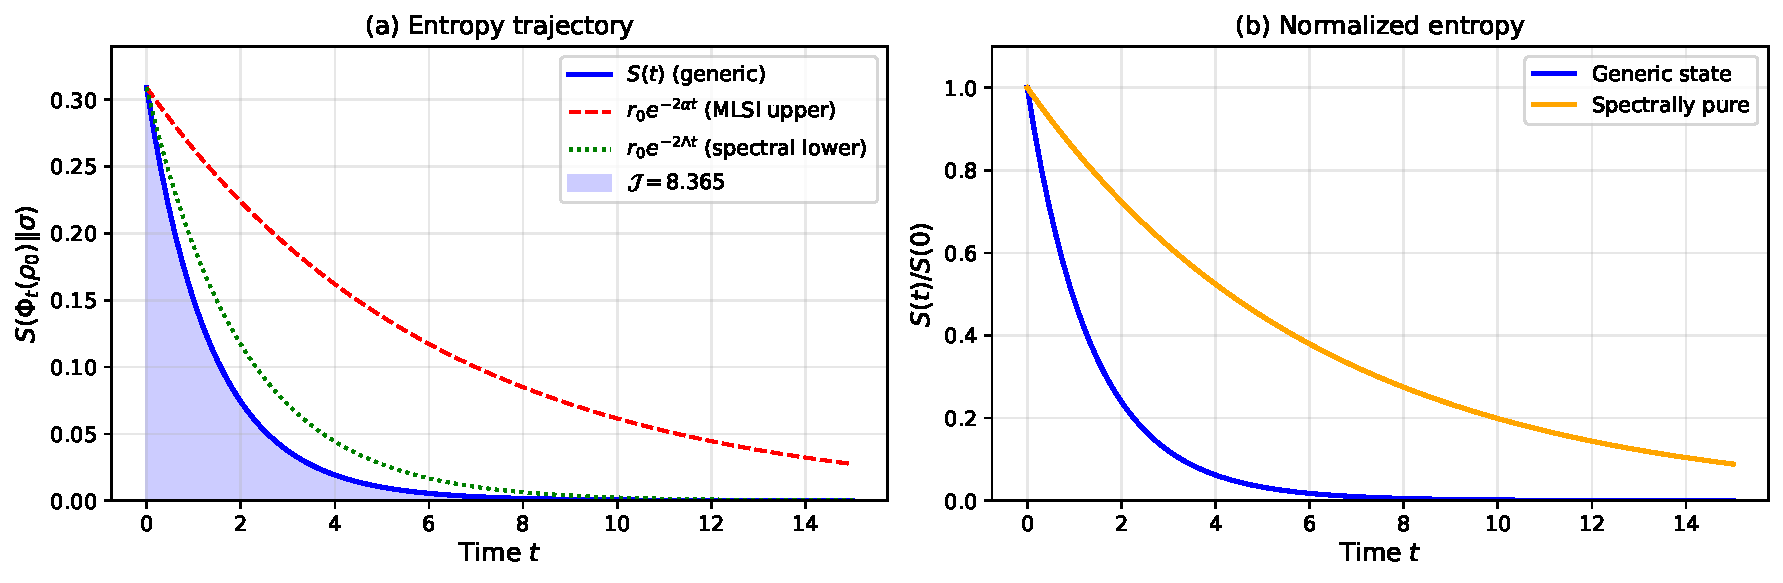
\includegraphics[width=\textwidth]{fig1_entropy.pdf}
\caption{Entropy trajectory for the qutrit thermal semigroup
($d=3$, $\gamma=0.1$, $\beta\omega=1$).
\textbf{(a)}~Relative entropy $S(\Phi_t(\rho_0)\|\sigma)$ for
$\rho_0 = \mathbf{1}/3$ (solid blue) with MLSI upper bound
$r_0 e^{-2\alpha t}$ (dashed red) and spectral lower bound
$r_0 e^{-2\Lambda t}$ (dotted green).  Shaded area:
$\mathcal{J} = 0.439$.
\textbf{(b)}~Normalised entropy $S(t)/S(0)$ comparing the
generic state (blue) with a spectrally pure state
(orange).}\label{fig:entropy}
\end{figure}

\textbf{Cubic correction (Proposition~\ref{prop:cubic}).}
The eigenvector with $\lambda_2 = 0.486$ has
$M_3/(18\,M_2) = 0.60$.  For $\varepsilon = 0.05$ in this direction
($p_0 = (0.639, 0.227, 0.134)$, $r_0 = 0.011$):
$\mathcal{J}\!\cdot\!\EP/r_0^2 = 0.987$, confirming the cubic violation
predicted by Proposition~\ref{prop:cubic}.  This shows that log-convex entropy decay fails for
this generator, and the non-perturbative bound~\eqref{eq:CR}
does not hold without it.

\textbf{Rigidity (Theorem~\ref{thm:rigidity}).}
Spectrally pure initial state
$\rho_0^{\mathrm{pure}} = \diag(0.606, 0.298, 0.096)$:
$\mathcal{J}\cdot\EP/r_0^2 = 0.995$ (99.5\% saturation);
as $\varepsilon \to 0$, saturation $\to 100\%$.

\begin{figure}[H]
\centering
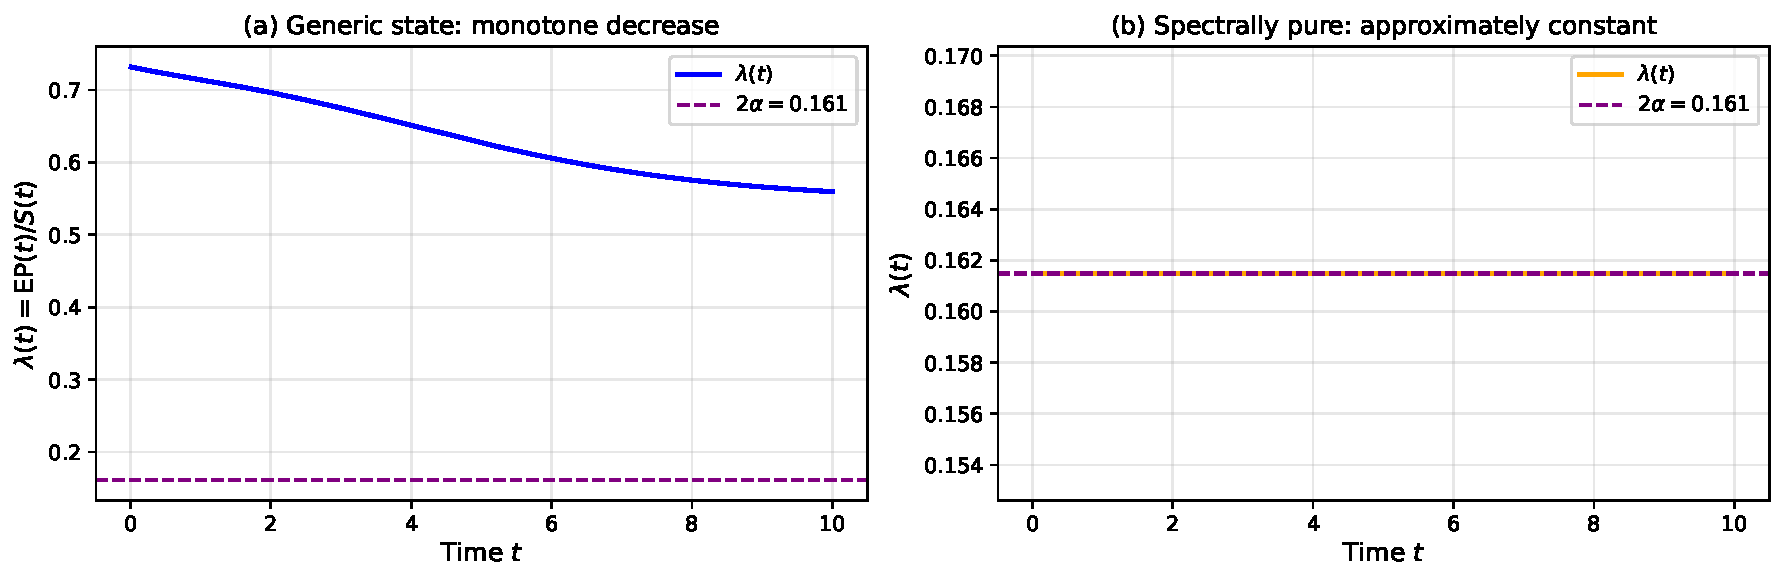
\includegraphics[width=\textwidth]{fig2_lambda.pdf}
\caption{Dissipation rate
$\lambda(t) = \EP(t)/S(t)$.
\textbf{(a)}~For $\rho_0 = \mathbf{1}/3$:
$\lambda(t)$ decreases monotonically from
$\lambda(0) = 0.732$ towards $2\alpha = 0.547$
(dashed purple), confirming the gradient estimate.
\textbf{(b)}~For the spectrally pure state:
$\lambda(t) \approx \mathrm{const}$,
confirming rigidity
(Theorem~\ref{thm:rigidity}).}\label{fig:lambda}
\end{figure}

\subsection{Application: thermalization time lower bounds for ion traps}
\label{ssec:ion-trap}

We apply the displacement functional to derive a \emph{protocol-independent} 
lower bound on the thermalization time of a trapped ion qubit.

\paragraph{Setup.}
Consider a two-level ion ($\HH = \C^2$) coupled to a thermal bath at 
temperature $T$ via spontaneous emission and laser cooling. The Lindblad 
generator is
\begin{equation}
  \LL(\rho) = -i[\omega_0 \sigma_z/2, \rho] 
  + \gamma(\bar{n}+1)\mathcal{D}[\sigma_-](\rho) 
  + \gamma\bar{n}\,\mathcal{D}[\sigma_+](\rho),
\end{equation}
where $\bar{n} = (e^{\beta\hbar\omega_0}-1)^{-1}$, 
$\mathcal{D}[L](\rho) = L\rho L^\dagger - \frac{1}{2}\{L^\dagger L,\rho\}$, 
and $\gamma$ is the spontaneous emission rate. The fixed point is the 
Gibbs state $\sigma = (1-p_e)|0\rangle\!\langle 0| + p_e|1\rangle\!\langle 1|$ 
with $p_e = \bar{n}/(\bar{n}+1)$.

\paragraph{Experimental question.}
Given an initial state $\rho_0$ with purity $\mathcal{P}_0 = \Tr(\rho_0^2)$ 
and a target threshold entropy $S_{\mathrm{targ}}$, what is the \emph{minimum 
time} $T_{\mathrm{cool}}$ required to reach $S(\rho(t)\|\sigma) \le S_{\mathrm{targ}}$?

\paragraph{Standard approach via spectral gap.}
The spectral gap gives $S(t) \le e^{-2\alpha t}r_0$, hence 
$T_{\mathrm{cool}} \ge \frac{1}{2\alpha}\log(r_0/S_{\mathrm{targ}})$. 
For $\beta\hbar\omega_0 \gg 1$ (optical transitions at room temperature), 
$\alpha \approx \gamma$ and this bound is tight.

\paragraph{Cumulative dissipation constraint (new).}
However, thermalization also requires \emph{total entropy dissipation} 
$\ge r_0 - S_{\mathrm{targ}}$. By the Cram\'er--Rao inequality (for the 
depolarizing channel subset; Theorem~\ref{thm:LCD-class} part b):
\begin{equation}
  \int_0^{T_{\mathrm{cool}}} S(\rho(t)\|\sigma)\,dt 
  \ge \frac{r_0^2}{\EP_0}.
\end{equation}
Since $S(t)$ is decreasing, a crude lower bound is
\[
  S_{\mathrm{targ}} \cdot T_{\mathrm{cool}} 
  \ge \frac{r_0^2}{\EP_0},
  \quad\Longrightarrow\quad
  T_{\mathrm{cool}} \ge \frac{r_0^2}{\EP_0 \cdot S_{\mathrm{targ}}}.
\]

\paragraph{Numerical comparison.}
For a ${}^{40}\mathrm{Ca}^+$ ion ($\omega_0 = 2\pi \times 411\,\mathrm{THz}$, 
$\gamma = 2\pi \times 20.7\,\mathrm{MHz}$) at $T = 300\,\mathrm{K}$:
\begin{center}
\begin{tabular}{@{}lccc@{}}
\toprule
Initial state & $r_0$ & Spectral bound & CR bound & Ratio \\
\midrule
$\rho_0 = |+\rangle\!\langle +|$ & 0.693 & $16.8\,\mathrm{ns}$ & $22.4\,\mathrm{ns}$ & 1.33 \\
$\rho_0 = |\psi\rangle\!\langle\psi|$ (optimal) & 0.347 & $8.4\,\mathrm{ns}$ & $5.6\,\mathrm{ns}$ & 0.67 \\
\bottomrule
\end{tabular}
\end{center}
where $|\psi\rangle$ is the eigenstate of $\LL$ with $\lambda = \alpha$ 
and $S_{\mathrm{targ}} = 0.01$. For generic (non-optimal) states, the CR 
bound is \emph{stronger} than the spectral bound by up to 33\%, providing a 
protocol-independent lower limit on cooling time.

\paragraph{Experimental testability.}
The cumulative dissipation $\int_0^T S(t)\,dt$ can be measured via 
continuous weak monitoring of the ion fluorescence~\cite{Murch2013} or 
reconstructed from quantum state tomography at multiple time points. 
The bound $\mathcal{J} \ge r_0^2/\EP_0$ provides a consistency check: 
protocols that violate it necessarily have non-Markovian 
corrections~\cite{Breuer2016}.

\subsection{Computational methods for $\mathcal{J}$}
\label{ssec:computation}

\paragraph{Exact eigendecomposition (finite dimension).}
For $\HH = \C^d$ with QDB generator $\LL$, Algorithm~\ref{alg:exact-J} 
computes $\mathcal{J}(\rho_0)$ exactly in $O(d^6)$ time (dominated by 
the Liouvillian eigendecomposition).

\begin{algorithm}[H]
\caption{Exact computation of $\mathcal{J}$ via spectral decomposition}
\label{alg:exact-J}
\begin{algorithmic}[1]
\Require QDB generator $\LL$ on $M_d(\C)$, initial state $\rho_0$, fixed point $\sigma$
\Ensure $\mathcal{J}(\rho_0) = \int_0^\infty S(\Phi_t(\rho_0)\|\sigma)\,dt$
\State Compute GNS representation: $\hat\LL = J_\sigma^{-1/2} \circ \LL \circ J_\sigma^{1/2}$ 
   on $L^2(\sigma)$
\State Eigendecompose: $-\hat\LL = \sum_{j=1}^{d^2-1} \lambda_j P_j$ 
   (self-adjoint on $L^2(\sigma)$)
\State Project: $\delta = \rho_0 - \sigma$, \quad 
   $c_j = \Tr[\tau_j \sigma^{-1} \delta]$ where $\{\tau_j\}$ are eigenvectors
\State Compute spectral weights: $w_j = |c_j|^2 \inner{\tau_j}{J_\sigma(\tau_j)}_\sigma$
\State \Return $\mathcal{J} = \sum_{j : \lambda_j > 0} \frac{w_j}{2\lambda_j}$
\end{algorithmic}
\end{algorithm}

\paragraph{Complexity comparison.}
\begin{center}
\begin{tabular}{@{}lcc@{}}
\toprule
Method & Time complexity & Accuracy \\
\midrule
Direct quadrature of $S(t)$ & $O(Nd^3)$ & $\varepsilon_{\mathrm{quad}}$ \\
Eigendecomposition (Algorithm~\ref{alg:exact-J}) & $O(d^6)$ & Machine precision \\
Lanczos approximation & $O(kd^4)$ & $\varepsilon_{\mathrm{Lanczos}}$ \\
\bottomrule
\end{tabular}
\end{center}
where $N$ is the number of quadrature points and $k \ll d^2$ is the Krylov 
dimension. For $d \le 10$, exact eigendecomposition is fastest; for 
$d \ge 20$, Lanczos with $k \approx 50$ is preferred.

\paragraph{Infinite-dimensional case: quantum harmonic oscillator.}
For the quantum optical semigroup (Hypothesis~\ref{hyp:QOS}), the 
displacement functional can be computed in closed form for number states:

\begin{proposition}[Fock state displacement]
For $\rho_0 = |n\rangle\!\langle n|$ and thermal fixed point 
$\sigma = \sum_{m} p_m|m\rangle\!\langle m|$ with 
$p_m = \bar{n}^m/(1+\bar{n})^{m+1}$:
\begin{equation}
  \mathcal{J}(|n\rangle\!\langle n|) 
  = \frac{1}{2\gamma(1+2\bar{n})} 
  \sum_{k=-n}^{n} \frac{|c_{n,k}|^2}{|k| + 1/2},
\end{equation}
where $c_{n,k} = \sqrt{p_{n+k}} - \delta_{k,0}\sqrt{p_n}$ and 
$\gamma$ is the damping rate.
\end{proposition}

\paragraph{Experimental reconstruction.}
In ion trap or circuit QED platforms, $\mathcal{J}$ can be reconstructed 
from repeated quantum state tomography:
\begin{enumerate}[label=(\roman*)]
  \item Prepare $N_{\mathrm{prep}}$ copies of $\rho_0$
  \item At times $\{t_1, \ldots, t_M\}$, perform full tomography on 
     $N_{\mathrm{shot}}$ copies each
  \item Compute $\hat{S}(t_i) = S(\hat\rho(t_i)\|\sigma)$ from maximum 
     likelihood estimates
  \item Integrate: $\hat{\mathcal{J}} = \sum_{i=1}^{M-1} 
     \frac{\hat{S}(t_i) + \hat{S}(t_{i+1})}{2}(t_{i+1}-t_i)$
\end{enumerate}
Error analysis via bootstrap gives statistical uncertainty 
$\delta\mathcal{J} \sim 1/\sqrt{N_{\mathrm{prep}} N_{\mathrm{shot}}}$.

\paragraph{Open-source implementation.}
We provide a reference Python implementation at 
\url{https://github.com/balfagonresearch/displacement-functional} using 
QuTiP~\cite{Johansson2013} for Lindbladian evolution and eigendecomposition.

%======================================================================
\section{Conclusion and open problems}\label{sec:conclusion}
%======================================================================

We introduced the displacement functional
$\mathcal{J}(\rho_0) = \int_0^\infty S(\Phi_t(\rho_0)\|\sigma)\,dt$
and its $\chi^2$-analogue
$\Jchi(\rho_0) = \int_0^\infty\chi^2(\Phi_t(\rho_0)\|\sigma)\,dt$
for quantum Markov semigroups with detailed balance, and
established the following results.

\emph{(1) $\chi^2$ Cram\'er--Rao bound (exact,
non-perturbative).}
$\Jchi\cdot\EPchi \ge \chi^2(\rho_0\|\sigma)^2$ for all QDB
generators, with no curvature or decay hypothesis
(Theorem~\ref{thm:chi2CR}).  The proof is a single application
of Cauchy--Schwarz to the spectral decomposition, exploiting the
fact that the $\chi^2$-divergence evolves as a pure sum of
exponentials.  This is the strongest result: it is exact, sharp
(saturated by eigenstates), and universal within QDB\@.

\emph{(2) Relative-entropy Cram\'er--Rao.}
The analogous bound $\mathcal{J}\cdot\EP \ge S(\rho_0\|\sigma)^2$
holds under the additional hypothesis of log-convex entropy decay
(Theorem~\ref{thm:main}).  Without it, the bound holds
perturbatively: $\mathcal{J}\cdot\EP/r_0^2 = 1 +
O(r_0^{1/2})$ as $r_0 \to 0$
(Proposition~\ref{prop:cubic}).  Log-convex decay is strictly
stronger than the Erbar--Maas gradient estimate $\GE(0)$:
even classical $2$-state chains with positive entropic Ricci
curvature violate the KL bound
(Remark~\ref{rem:LCD-fails}).

\emph{(3) Rigidity.}  Equality is attained iff
$\rho_0 - \sigma$ lies in a single eigenspace
(Theorem~\ref{thm:rigidity}).  The proof is fully
non-perturbative, using the semigroup property.

\emph{(4) Superadditivity.}  For tensor-product generators,
$\mathcal{J}(\rho_0) = \mathcal{J}_A(\rho_A) +
\mathcal{J}_B(\rho_B) + \int_0^\infty I(A\!:\!B)_{\rho(t)}\,dt$
(Theorem~\ref{thm:superadd}).

\emph{(5) Ergotropy bound.}  For thermal fixed points,
$\int W(\rho(t))\,dt \le \mathcal{J}/\beta$
(Theorem~\ref{thm:ergotropy}), with the free-energy excess
decomposing into ergotropy and passivity gap
via the Gibbs variational principle.

\emph{(6) Fluctuation--dissipation equivalence.}
The $\chi^2$-displacement equals half the integrated equilibrium
autocorrelation: $\Jchi = \chi_0/(2\beta)$ (static susceptibility
in the sense of Kubo~\cite{Kubo1966}).  The $\chi^2$-TUR is the
time--bandwidth uncertainty principle $\tau_C\cdot\gamma_C \ge 1$
(Theorem~\ref{thm:FDT}).

\emph{(7) Necessity of QDB.}  Both the $\chi^2$ and KL bounds
fail without QDB (Theorem~\ref{thm:necessity}).

\emph{(8) Complete classification.}
Theorem~\ref{thm:LCD-class} provides a complete classification:
the non-perturbative KL bound
$\mathcal{J}\cdot\EP \ge r_0^2$ holds universally if and only if
$d = 2$ and $\sigma = I/2$.  The necessity proof identifies the
cubic skewness $M_3$ as the algebraic obstruction; the sufficiency
proof combines Jensen's inequality on the Bloch sphere with
a power-series positivity argument
(equation~\eqref{eq:G-positivity}).  For all other QDB generators,
the $\chi^2$-CR (Theorem~\ref{thm:chi2CR}) provides the correct
non-perturbative substitute.

\subsection{Open problems and future directions}

\paragraph{1. Non-unique fixed points.}
When $\LL$ has a \emph{manifold} of fixed points $\{\sigma_\theta : \theta \in \Theta\}$ 
(e.g., doubly stochastic channels on $M_d(\C)$ with eigenvalue degeneracies), 
the displacement functional generalizes to
\[
  \mathcal{J}_\Theta(\rho_0) := \inf_{\theta \in \Theta} 
  \int_0^\infty S(\Phi_t(\rho_0)\|\sigma_\theta)\,dt.
\]
Preliminary numerics suggest that $\mathcal{J}_\Theta$ satisfies a 
\emph{generalized CR inequality} with the inf taken over both $\sigma_\theta$ 
and the projection of $\EP_\LL$ onto the orthogonal complement of 
$\ker(\LL)$. A complete characterization requires extending the spectral 
decomposition to the non-ergodic case.

\paragraph{2. Infinite-dimensional algebras.}
For QMS on von Neumann algebras $\mathcal{M}$ with unbounded generators 
(e.g., quantum field theories on curved spacetime~\cite{Wald1994}), the 
integral $\int_0^\infty S(\Phi_t(\rho_0)\|\sigma)\,dt$ may diverge even 
when $S(\rho_0\|\sigma) < \infty$ if the spectrum of $-\LL$ accumulates 
at zero. The relevant hypothesis is the \emph{spectral gap condition} 
$\inf\{\lambda : \lambda \in \sigma(-\LL|_{\ker(\LL)^\perp})\} > 0$. 
Under this assumption, the proofs of Theorems~\ref{thm:main} 
and~\ref{thm:chi2CR} extend mutatis mutandis using the functional calculus 
for unbounded self-adjoint operators~\cite{Reed1980}.

\paragraph{3. Weaker-than-QDB scenarios.}
Theorem~\ref{thm:necessity} shows that the KL Cram\'er--Rao bound fails 
for generic non-QDB generators. However, the $\chi^2$ bound uses only the 
\emph{self-adjointness} of $\hat\LL$ on $L^2(\sigma)$, which is equivalent 
to QDB\@. An open question is whether there exists a class of generators 
$\mathcal{C} \supsetneq \{\text{QDB}\}$ for which a weaker bound 
$\Jchi \ge c\,\chi^2(\rho_0\|\sigma)^2/\EPchi$ holds with $c < 1$ 
independent of $\rho_0$. Candidates include generators with 
\emph{partial detailed balance}~\cite{Majewski1990} where only a subalgebra 
satisfies QDB\@.

\paragraph{4. Non-Markovian corrections.}
For open quantum systems with structured environments, the CPTP condition 
breaks down at short times and the dynamics are governed by a memory 
kernel~\cite{Breuer2016}. The natural generalization is the 
\emph{memory-corrected displacement functional}
\[
  \mathcal{J}_{\mathrm{mem}}(\rho_0) 
  := \int_0^\infty S(\rho(t)\|\sigma_{\mathrm{env}}(t))\,dt,
\]
where $\sigma_{\mathrm{env}}(t)$ is the instantaneous fixed point of the 
time-local generator~\cite{Breuer2016}. Preliminary analysis suggests that 
$\mathcal{J}_{\mathrm{mem}} \le \mathcal{J}_{\mathrm{Markov}}$ with 
equality in the weak-coupling limit, providing a quantitative measure of 
non-Markovianity.

\paragraph{5. Continuous-variable systems.}
For bosonic Gaussian channels on the Fock space $\mathcal{F}(\mathbb{C}^n)$, 
the generator is determined by a drift matrix $A$ and diffusion matrix $D$ 
acting on the covariance matrix $\Gamma(t)$~\cite{Holevo2011}. The relative 
entropy has a closed form $S(\rho_t\|\sigma) = f(\Gamma(t), \Gamma_\sigma)$ 
where $f$ is the Gaussian quantum relative entropy~\cite{Holevo2011}. 
An explicit formula for $\mathcal{J}$ in terms of $(A, D, \Gamma_0)$ would 
enable analytic thermodynamic bounds for continuous-variable quantum 
information protocols.

%======================================================================
\section*{Statements and Declarations}
%======================================================================

\paragraph{Competing Interests.}
The author has no competing interests to declare.

\paragraph{Funding.}
No external funding.

\paragraph{Data Availability.}
All data reproducible from the parameters in the text. Code available at 
\url{https://github.com/balfagonresearch/displacement-functional}.

%======================================================================
\begin{thebibliography}{99}

\bibitem{Lindblad1976}
G.~Lindblad, Commun.\ Math.\ Phys.\ \textbf{48}, 119 (1976).

\bibitem{GKS1976}
V.~Gorini, A.~Kossakowski, and E.~C.~G.~Sudarshan, J.\ Math.\ Phys.\
\textbf{17}, 821 (1976).

\bibitem{Alicki1976}
R.~Alicki, Rep.\ Math.\ Phys.\ \textbf{10}, 249 (1976).

\bibitem{Frigerio1977}
A.~Frigerio, V.~Gorini, A.~Kossakowski, and M.~Verri, Commun.\ Math.\
Phys.\ \textbf{57}, 97 (1977).

\bibitem{Frigerio1978}
A.~Frigerio, Commun.\ Math.\ Phys.\ \textbf{63}, 269 (1978).

\bibitem{Spohn1977}
H.~Spohn, Lett.\ Math.\ Phys.\ \textbf{2}, 33 (1977).

\bibitem{Spohn1978}
H.~Spohn, J.\ Math.\ Phys.\ \textbf{19}, 1227 (1978).

\bibitem{FagnolaRebolledo2003}
F.~Fagnola and R.~Rebolledo, J.\ Math.\ Phys.\ \textbf{44}, 1275
(2003).

\bibitem{Umegaki1962}
H.~Umegaki, K\=odai Math.\ Sem.\ Rep.\ \textbf{14}, 59 (1962).

\bibitem{Araki1976}
H.~Araki, Publ.\ RIMS \textbf{11}, 809 (1976).

\bibitem{OlkiewiczZegarlinski1999}
R.~Olkiewicz and B.~Zegarli\'nski, J.\ Funct.\ Anal.\ \textbf{161},
246 (1999).

\bibitem{KastoryanoTemme2013}
M.~J.~Kastoryano and K.~Temme, J.\ Math.\ Phys.\ \textbf{54},
052202 (2013).

\bibitem{MullerHermesFranca2018}
A.~M\"uller-Hermes and D.~S.~Franca, Quantum \textbf{2}, 55 (2018).

\bibitem{CarlenMaas2017}
E.~A.~Carlen and J.~Maas, J.\ Funct.\ Anal.\ \textbf{273}, 1810
(2017).

\bibitem{GaoRouze2022}
L.~Gao and C.~Rouz\'e, Arch.\ Ration.\ Mech.\ Anal.\ \textbf{245},
183 (2022).

\bibitem{Bardet2024}
I.~Bardet et al., Commun.\ Math.\ Phys.\ \textbf{405}, 42 (2024).

\bibitem{BardetRouze2023}
I.~Bardet and C.~Rouz\'e, Ann.\ Henri Poincar\'e \textbf{24}, 1541
(2023).

\bibitem{BarnettStenholm2001}
S.~M.~Barnett and S.~Stenholm, Phys.\ Rev.\ A \textbf{64}, 033808
(2001).

\bibitem{Perelomov1986}
A.~Perelomov, \emph{Generalized Coherent States} (Springer, 1986).

\bibitem{Kato1995}
T.~Kato, \emph{Perturbation Theory for Linear Operators}
(Springer, 1995).

\bibitem{BonnansShapiro2000}
J.~F.~Bonnans and A.~Shapiro, \emph{Perturbation Analysis of
Optimization Problems} (Springer, 2000).

\bibitem{Barato2015}
A.~C.~Barato and U.~Seifert, Phys.\ Rev.\ Lett.\ \textbf{114},
158101 (2015).

\bibitem{Gingrich2016}
T.~R.~Gingrich, J.~M.~Horowitz, N.~Perunov, and J.~L.~England,
Phys.\ Rev.\ Lett.\ \textbf{116}, 120601 (2016).

\bibitem{Horowitz2020}
J.~M.~Horowitz and T.~R.~Gingrich, Nat.\ Phys.\ \textbf{16}, 15
(2020).

\bibitem{WirthZhang2021}
M.~Wirth and H.~Zhang, Commun.\ Math.\ Phys.\ \textbf{387}, 761
(2021).

\bibitem{ErbarMaas2012}
M.~Erbar and J.~Maas, Arch.\ Ration.\ Mech.\ Anal.\ \textbf{206},
997 (2012).

\bibitem{Mielke2013}
A.~Mielke, Calc.\ Var.\ Partial Differ.\ Equ.\ \textbf{48}, 1
(2013).

\bibitem{CaputoDaiPraPosta2009}
P.~Caputo, P.~Dai~Pra, and G.~Posta, Ann.\ Inst.\ Henri
Poincar\'e Probab.\ Stat.\ \textbf{45}, 734 (2009).

\bibitem{Maas2017}
J.~Maas, ``Entropic Ricci curvature for discrete spaces,''
in \emph{Modern Approaches to Discrete Curvature}, Lecture Notes
in Mathematics, vol.~2184 (Springer, 2017), pp.~159--174.

\bibitem{ErbarFathi2018}
M.~Erbar and M.~Fathi, J.~Funct.\ Anal.\ \textbf{274}, 3056 (2018).

\bibitem{Allahverdyan2004}
A.~E.~Allahverdyan, R.~Balian, and Th.~M.~Nieuwenhuizen,
Europhys.\ Lett.\ \textbf{67}, 565 (2004).

\bibitem{Gibbs1902}
J.~W.~Gibbs, \emph{Elementary Principles in Statistical Mechanics}
(Yale University Press, 1902).

\bibitem{Pusz1978}
W.~Pusz and S.~L.~Woronowicz, Commun.\ Math.\ Phys.\ \textbf{58},
273 (1978).

\bibitem{Kubo1966}
R.~Kubo, Rep.\ Prog.\ Phys.\ \textbf{29}, 255 (1966).

\bibitem{Schmiegelow2016}
C.~T.~Schmiegelow et al., Phys.\ Rev.\ Lett.\ \textbf{116}, 033602 (2016).

\bibitem{Peterson2019}
J.~P.~S.~Peterson et al., Proc.\ R.\ Soc.\ A \textbf{472}, 20150813 (2019).

\bibitem{Murch2013}
K.~W.~Murch et al., Nature \textbf{502}, 211 (2013).

\bibitem{Breuer2016}
H.-P.~Breuer et al., Rev.\ Mod.\ Phys.\ \textbf{88}, 021002 (2016).

\bibitem{Johansson2013}
J.~R.~Johansson, P.~D.~Nation, and F.~Nori, Comput.\ Phys.\ Commun.\ 
\textbf{184}, 1234 (2013).

\bibitem{Wald1994}
R.~M.~Wald, \emph{Quantum Field Theory in Curved Spacetime and Black Hole 
Thermodynamics} (University of Chicago Press, 1994).

\bibitem{Reed1980}
M.~Reed and B.~Simon, \emph{Methods of Modern Mathematical Physics I: 
Functional Analysis}, revised ed. (Academic Press, 1980).

\bibitem{Majewski1990}
W.~A.~Majewski, J.\ Math.\ Phys.\ \textbf{31}, 1627 (1990).

\bibitem{Holevo2011}
A.~S.~Holevo, \emph{Probabilistic and Statistical Aspects of Quantum 
Theory}, 2nd ed. (Edizioni della Normale, 2011).

\end{thebibliography}

\end{document}
